\documentclass[12pt,a4paper]{article}
\usepackage{hyperref}
\usepackage{graphicx}
\title{Laboratory 2: Unauthorized Access in Wireless Networks}
\author{Niclas Scheuing and Vasileios Dimitrakis}
\begin{document}
	\maketitle
	
	\section{Introduction}
	
	
	\section{Materials and Methods}
	Throughout the lab exercise 2 we used different materials and methods, that are presented below:
	
	\begin{itemize}
		\item \emph{MATLAB}: Vector- and numerical computing environment.
	\end{itemize}
	
	\section{Terminology}
	
	
	\section{Tasks}
	
	\section{Questions}
		\subsection{System configuration}
			Length of message
			Length of code
			chips per symbol
			processing gain
		
		\subsection{Jamming resistance of DSSS}
			Below noise
			multiband
			
		\subsection{Security introduced by DSSS}
		
		\subsection{}
	
	
	\begin{figure}
		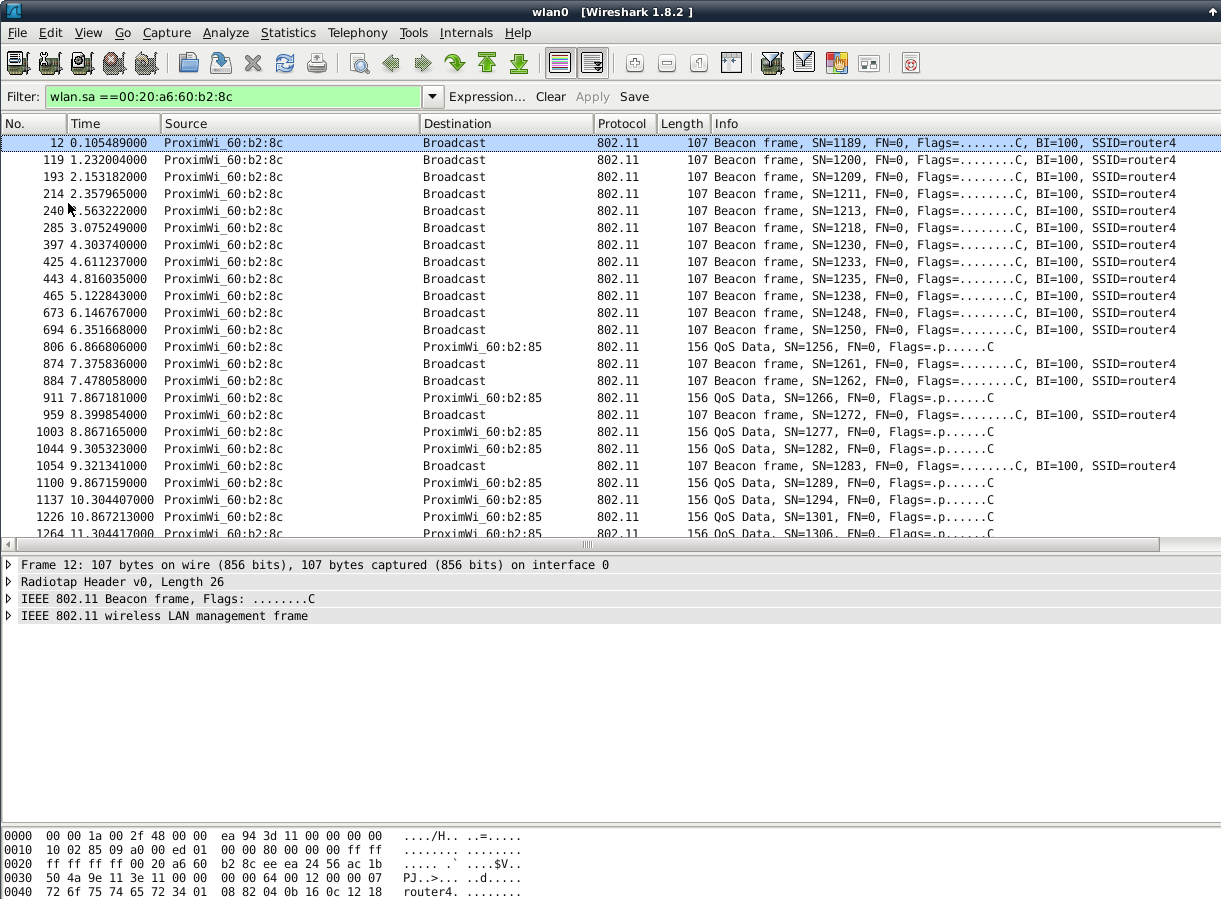
\includegraphics[width=\textwidth]{images/bill/pic1.png}
		\caption{Capturing the traffic using source \emph{MAC} address filtering.}
		\label{wep:wireshark}
	\end{figure}
	
	\section{Analysis}
	In this lab we demonstrated that some widely used security mechanisms as MAC-filtering, WEP and WPA2 are prone to rather simple 
	
	
	\bibliographystyle{plain}
	\bibliography{bibliography}
\end{document}\grid
